%! TEX program = xelatex
\documentclass[25pt, a0paper, portrait, margin=0mm, innermargin=25mm,
blockverticalspace=15mm, colspace=15mm, subcolspace=8mm]{tikzposter}

\usepackage{wrapfig}
\usepackage[no-math]{fontspec}      

\settitle{%
	\begin{minipage}{0.2\linewidth}
		\centering
		\@titlegraphic
	\end{minipage}%
	\begin{minipage}{0.8\linewidth}
		\centering
		\color{titlefgcolor}
		{
			\bfseries \Huge \sc \@title
		}
		\\
		\vspace*{2em}
		{
			\begin{minipage}{0.4\linewidth}
				\centering
				\large Aufar Gilbran\\%
				\large aufargilbran@gmail.com
			\end{minipage}%
			\begin{minipage}{0.5\linewidth}
				\centering
				\large Achmad Imam Kistijantoro\\%
				\large imam@stei.itb.ac.id
			\end{minipage}
		}
	\end{minipage}%
}

\definebackgroundstyle{my}{}
\definetitlestyle{my}{
	width=820mm,
	titletotopverticalspace=20mm, titletoblockverticalspace=30mm,
	titlegraphictotitledistance=90pt
}{}

\definelayouttheme{my}{
	\usebackgroundstyle{my}
	\usetitlestyle{my}
}

\usetheme{my}


\title{\parbox{\linewidth}{
		\centering%
Improving ARINC 653 Systems Reliability by Using Fault-Tolerant Partition Scheduling}}
\titlegraphic{
\includegraphics[width=10cm]{logo-itb.png}}

\begin{document}
\maketitle
\block{Introduction}{
	The ARINC 653 specifies multiple operating system components to
	provide isolation between partitions in avionics. This means
	failure on one partition in such system does not affect any
	other partition.  While each partition cannot affect the other
	partitions, the failure still happens and possibly leads to
	failure to the whole system. System failure on avionics often
	leads to significant increase of the safety risk for the people
	and/or environment involved.

	Currently, solutions for described problem already exists and
	implemented. Unfortunately, these solutions are proprietary, thus
	limiting further research for this domain. This research will
	propose a reliable ARINC 653 compliant system which will be
	provided gratis for further research.

}
\begin{columns}
	\column{0.4}
	\block{ARINC 653}{
		The primary goal of ARINC 653 specification is to manage contended resources across many domains
		with safety and fault isolation for users of these
		resources. Isolation (or commonly referred as
		partition) is done on basic subsystem resources,
		including, but not limited to, CPU time, memory,
		and I/O bandwidth. These partitioning is
		already implemented on ARLX.
	}
	\column{0.6}
	\block{Improving System Reliability}{
		To improve service reliability in real-time systems, one
		solution is to have the scheduler to be fault-tolerant. Studies
		shows that a hierarchical scheduler like ARINC 653 scheduler
		can be made fault-tolerant by means of primary-backup scheme.

		Primary-backup scheme will be used when choose partition to
		run. If primary partition experienced a failure, a backup
		partition is chosen to run in place of the faulty primary
		partition.

	}
\end{columns}

\block{ARINC 653 Scheduler}
{
	ARINC 653 specification specifies two type of scheduler, partition scheduler and process
	scheduler. Partition scheduling is used to schedule which partitions should be given the CPU
	time at current time. Process scheduling is used to schedule which process inside the partition
	should be given the VCPU time at current time. In this paper, we interchange the term partition
	scheduler with scheduler since we will not use process scheduler that much. Each of these
	schedulers works on a different context. The partition scheduler is a periodically repeating
	fixed timeslice scheduler for partitions. Every partition to be scheduled has their own fixed
	timeslice. So the partition will be activated at a certain time window. This window is called
	minor frame. The partition scheduling algorithm is predetermined, repetitive with a fixed
	periodicity. This period is called the major time frame. The major time frame should be big
	enough to run all the minor frame to be scheduled. Each partition can be configured to take at
	least one the time-slot within the major time frame. Partitions do not have a priority assigned
	to them so there is no preemption within the scheduling algorithm except for system calls
	(hypercalls in hypervisor context) or interrupts.

	\centering
	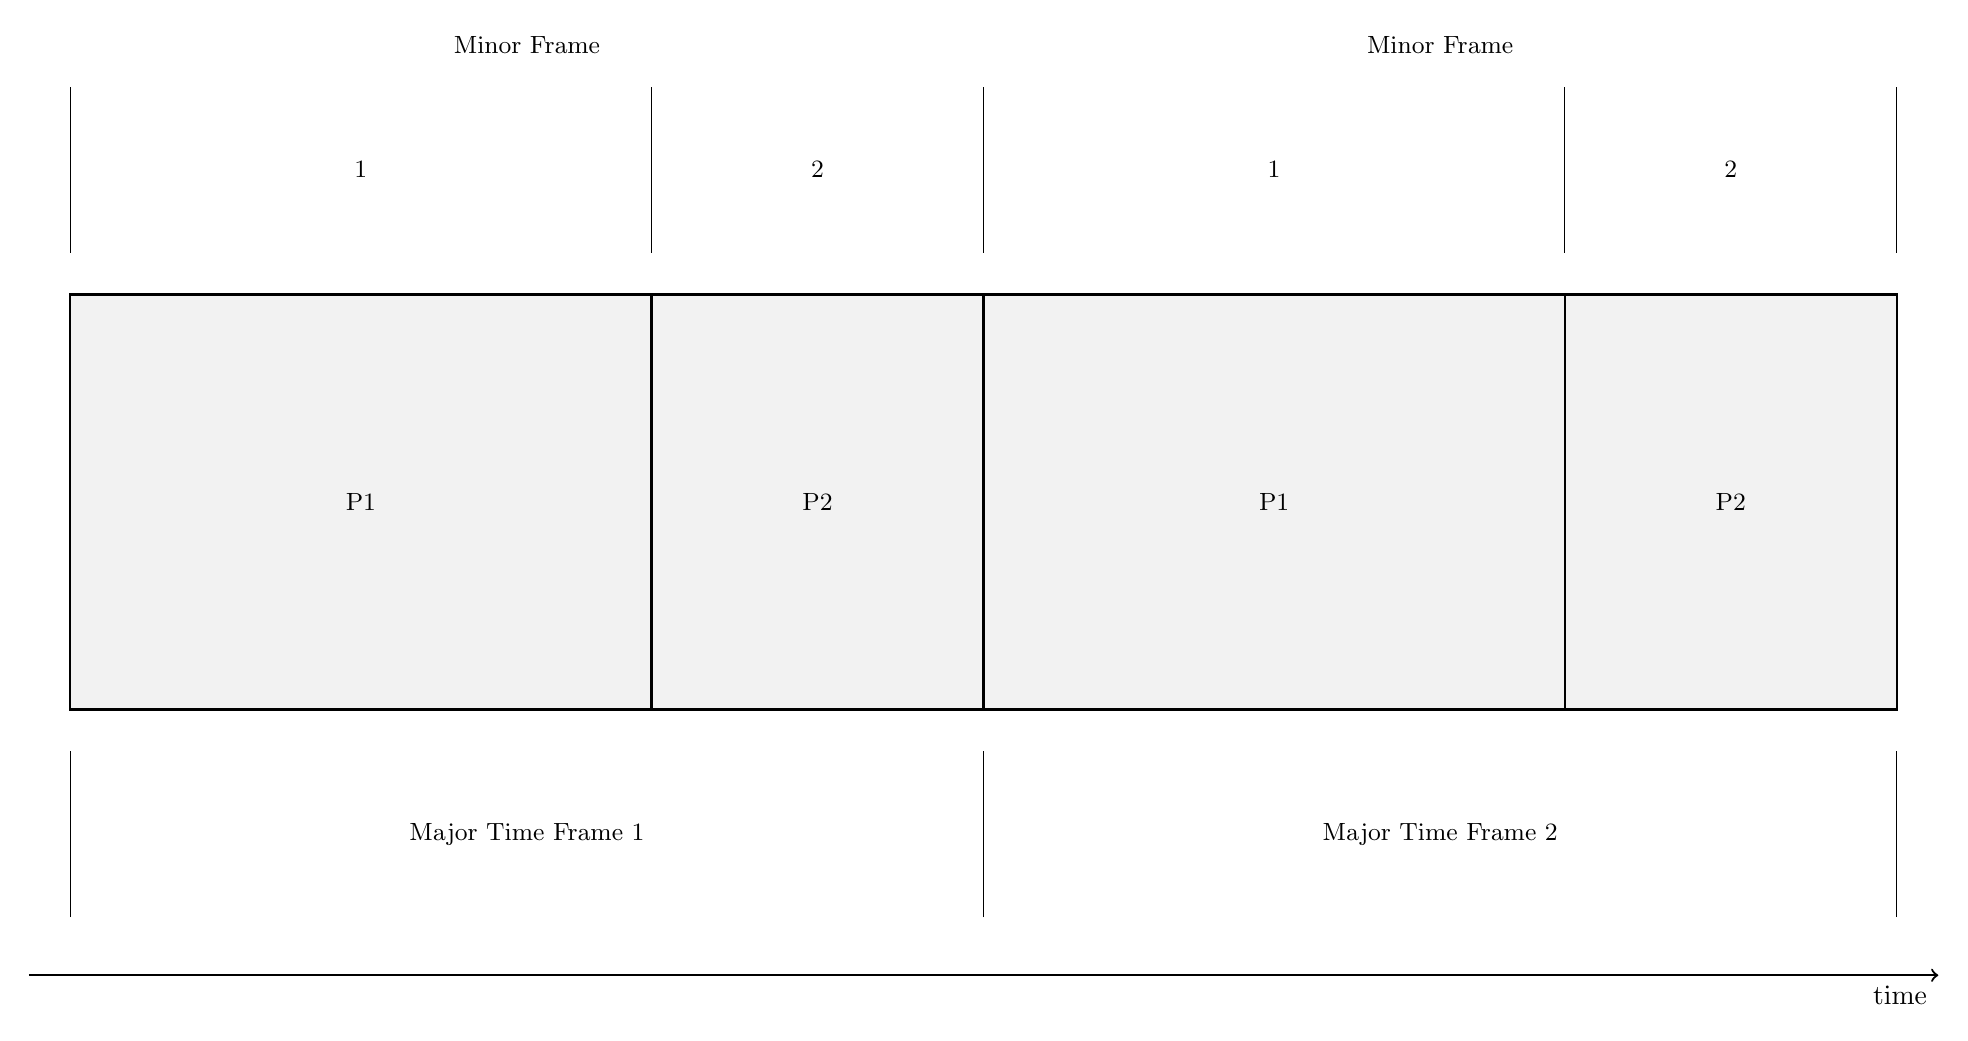
\begin{tikzpicture}[scale=3.0]
		{
			\def\boxh{50pt}
			\def\lineh{20pt}
			\def\off{110pt}
			\def\nodestyle{node[pos=0.5,font=\small]}
				\foreach \o in {0,...,1}
				{
					\pgfmathtruncatemacro{\mtlabel}{\o + 1}

					\path (\off*\o+00pt, \boxh+\lineh+10pt) -- ++(\off, 0pt) \nodestyle {Minor Frame};
					\draw (\off*\o+00pt, \boxh+5pt) -- ++(0pt, \lineh);
					\path (\off*\o+00pt, \boxh+5pt) -- ++(70pt, \lineh) \nodestyle
						(min\o) {1};

					\draw (\off*\o+70pt, \boxh+5pt) -- ++(0pt, \lineh);
					\path (\off*\o+70pt, \boxh+5pt) -- ++(40pt, \lineh) \nodestyle (min\o) {2};

					\draw (\off*\o+\off, \boxh+5pt) -- ++(0pt, \lineh);

					\draw[thick, fill=gray, fill opacity=0.10, text opacity=1.0] (\off*\o+00pt,0pt) rectangle +(70pt,\boxh) \nodestyle {P1};
					\draw[thick, fill=gray, fill opacity=0.10, text opacity=1.0] (\off*\o+70pt,0pt) rectangle +(40pt,\boxh) \nodestyle {P2};

					\path (\off*\o+0pt,-\lineh-5pt) -- ++(\off, \lineh) \nodestyle (mt\o) {Major Time
						Frame \mtlabel};
					\draw (\off*\o+0pt,-\lineh-5pt) -- ++(0pt, \lineh);
					\draw (\off*\o+\off,-\lineh-5pt) -- ++(0pt, \lineh);
				}
				\draw[thick, ->] (-5pt,-\lineh-12pt) -- (2*\off+5pt, -\lineh-12pt)
					node[pos=0.98,below] {time};
			}
		\end{tikzpicture}
}

\block{The Scheduling Strategy}{
	To keep the scheduling deterministic, we need to make sure that the algorithm will not depend on
	external sources. The input of the scheduling algorithm is partition information which already
	discussed in the last part. The scheduler selects one of the runnable partition such that its
	status is healthy and there are no partitions that have provided the service corresponding to
	its service identification. When the scheduler scans the schedule list, we extend it to also
	check whether the partition satisfies said conditions.

	It is trivial to check whether the partition is healthy. To check whether the service it
	provides have been provided before, we need a flag for possible service identification value.
	The flag is initialized to zero for all services at first. When a partition already exhausted
	its quantum, the scheduler then toggle the flag for the corresponding service. This is feasible
	without changing the required space complexity for the scheduler. Since service identification
	value corresponds to partition identification, thus its value is incremental from $1$ to $N$
	with $N$ is the number of partitions available. Thus, the extra space in the scheduler we need
	for the flag is linear to the number of partitions, which is the same as the schedule list
	itself.

	At the end of the major time frame, this algorithm ensures that given a service will be provided
	if there is at least one partition providing the service that is healthy. The algorithm will
	restart this process if current major time frame is elapsed. This whole process will be done
	indefinitely.
}

\end{document}
